% !TeX root = ../TFG_LaTeX.tex
\section{Lema de Schwarz i automorfismes del disc}

\begin{adjustwidth}{1cm}{1cm}

El Lema de Schwarz és un dels resultats fonamentals en l'estudi de les aplicacions holomorfes del disc unitat en si mateix. Proporciona una informació molt precisa sobre el comportament d'aquestes funcions quan fixen l'origen: no poden augmentar el mòdul dels punts i, en el cas d'igualtat, la funció ha de ser necessàriament una rotació.

Aquest resultat permet entendre millor l'estructura dels automorfismes del disc unitat. En particular, combinant el Lema de Schwarz amb certes transformacions de Möbius que envien punts del disc en l'origen, s'obté una descripció explícita de tots els automorfismes de $\mathbb{D}$. Aquestes funcions tindran un paper central al llarg de la secció, ja que permeten introduir de manera natural la mètrica pseudohiperbòlica i estudiar les aplicacions holomorfes del disc des d'un punt de vista geomètric.

La generalització natural d'aquest resultat és el Lema de Schwarz-Pick, que mostra que tota funció holomorfa $f : \mathbb{D} \to \mathbb{D}$ és una contracció respecte de la mètrica pseudohiperbòlica. Això permet distingir clarament els automorfismes del disc com aquelles aplicacions que preserven exactament aquesta distància. Finalment, introduirem els productes de Blaschke finits, que constitueixen una família important de funcions holomorfes del disc relacionades amb les propietats de preservació de la frontera $\partial \mathbb{D}$.

Per a una exposició més detallada del Lema de Schwarz, dels automorfismes del disc i del Lema de Schwarz-Pick, es poden consultar les referències \cite[Cap. IX]{gamelin} i \cite[Cap. 4]{shapiro}. Per als productes de Blaschke, es pot consultar també \cite[Cap. 15]{rudin}.

\begin{subsection}{Lema de Schwarz}

\begin{lema}[Schwarz]
    Siga $f(z)$ una funció holomorfa en $\mathbb{D}$. Suposem que $|f(z)|\leq 1$ per a tot $z\in\mathbb{D}$, i que a més, $f(0)=0$. Aleshores, 
    \begin{equation}
        |f(z)|\leq |z| \text{ per a tot } z\in\mathbb{D}.
        \label{LemaSchwarz}
    \end{equation} 
    A més, si es dóna la igualtat en l'equació (\ref{LemaSchwarz}) per a algun punt en $\mathbb{D}^*$, aleshores es té que $f(z)=\lambda z$ per a algun $\lambda \in \partial \mathbb{D}$. 
\end{lema}

\begin{proof}
    Primerament, considerem la funció $g(z)$ definida en $\mathbb{D}$
    \[
        g(z)=
        \begin{cases}
            \frac{f(z)}{z} &\text{ si } z\neq 0 \\
            f'(0) &\text{ si } z=0
        \end{cases}.
    \]
    Aquesta funció és holomorfa en $\mathbb{D}$ perquè és holomorfa en $\mathbb{D}\backslash\{0\}$ per ser $f$ holomorfa, i a més la singularitat que té en el $0$ és evitable, i el límit és $f'(0)$, ja que $\displaystyle\lim_{z\to 0}f(z)/z=f'(0)=:g(0)$.

    A continuació, considerem $0<r<1$, i siga $z\in \mathbb{D}^*$ tal que $|z|=r$. Es té que $|g(z)|=|f(z)|/r\leq 1/r$. Aplicant ara el Teorema del Mòdul Màxim (Teorema \ref{teo_mod_max}), obtenim que $|g(z)|\leq \frac{1}{r}$ en $\overline{B(0,r)}$. Si fem tendir $r \to 1$, aleshores obtenim que $|g(z)| \leq 1$ en $\mathbb{D}$. Això vol dir, si tenim en compte que $f(0)=0$, que $|f(z)|\leq|z|$ en $\mathbb{D}$, i tenim la primera part del lema.

    Ara suposem que existeix $z_0\in \mathbb{D}^*$ tal que $|f(z_0)|=|z_0|$. Aleshores $|g(z_0)|=1$, i altra vegada pel Teorema del Mòdul Màxim, tenim que $g(z)=\lambda\in \mathbb{C}$ tal que $|\lambda|=1$. Per tant, tenint en compte que $f(0)=0$, es té que $f(z)=\lambda z$.

\end{proof}

\begin{figure}[H]
    \centering
    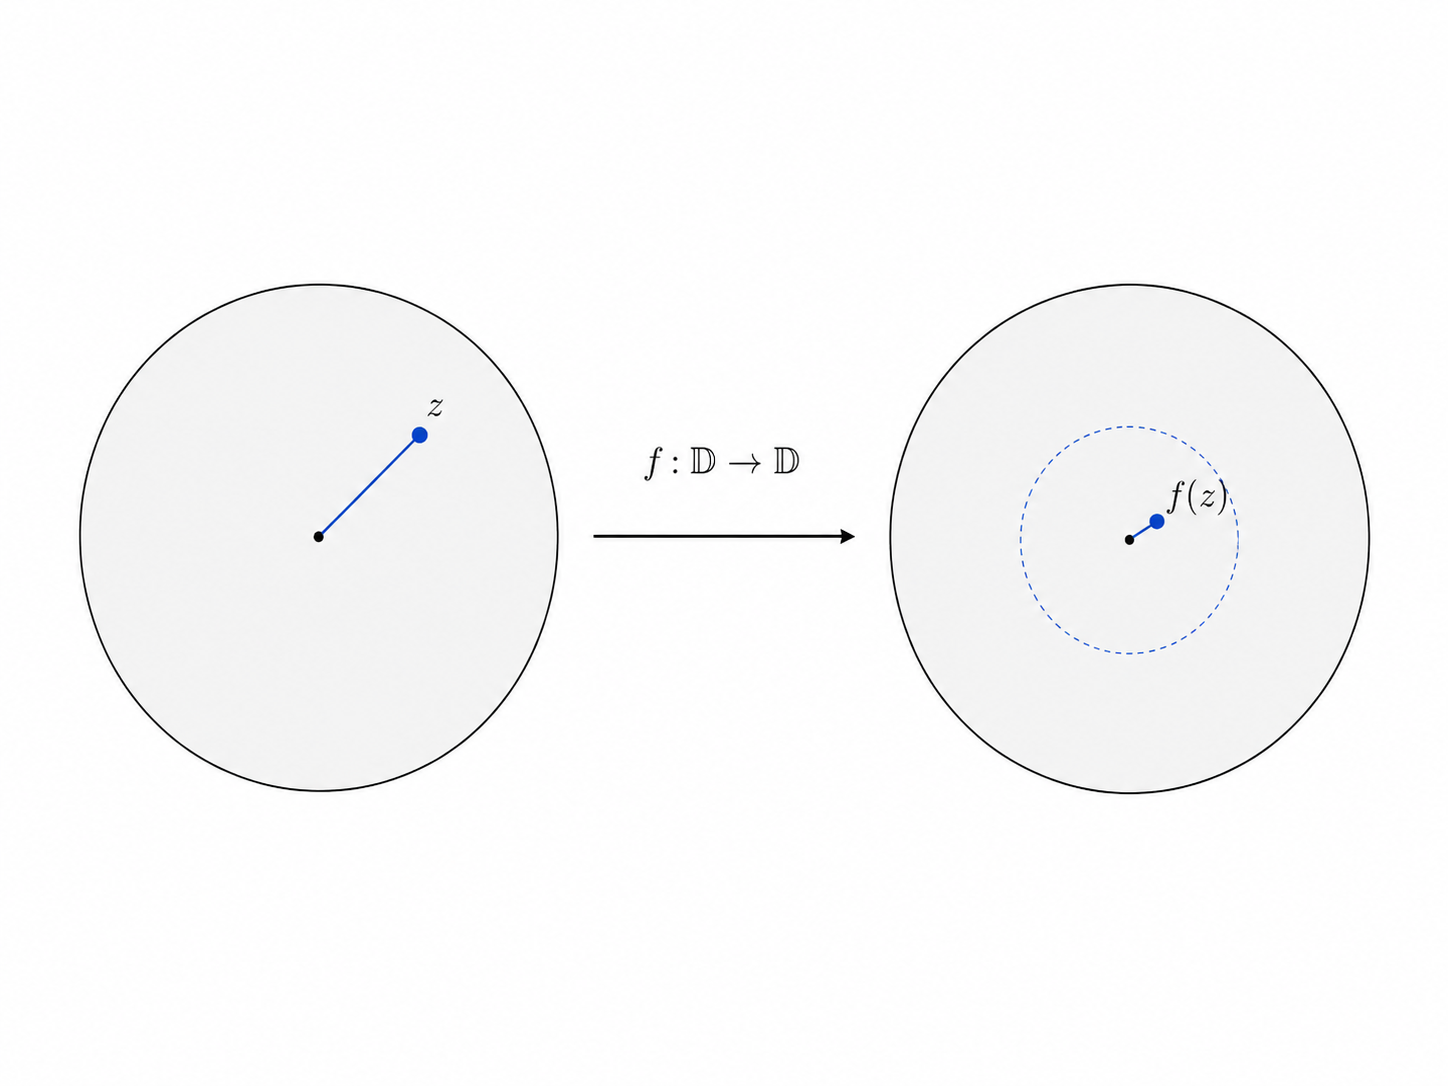
\includegraphics[width=0.55\textwidth]{pictures/Lema_Schwarz.png}
    \begin{adjustwidth}{1cm}{1cm}
       \caption{Representació del Lema de Schwarz.}
    \label{fig:schwarz} 
    \end{adjustwidth}
\end{figure}

Existeix també una versió per a la derivada del Lema de Schwarz.

\begin{lema} Siga $f(z)$ una funció holomorfa en $\mathbb{D}$. Si $|f(z)|\leq 1$ per a tot $z\in \mathbb{D}$, i a més $f(0)=0$, aleshores
    \begin{equation}
        |f'(0)|\leq 1,
        \label{eq_schwarz_lema_2}
    \end{equation}

i la igualtat es dóna si i només si $f(z)=\lambda z$ per a alguna constant $\lambda$ amb $|\lambda|=1$.
\label{LemaSchwarz_2}
\end{lema}

\begin{proof}
    Per a obtindre l'equació (\ref{eq_schwarz_lema_2}), simplement hem de fer tendir $z\to 0$ en el lema de Schwarz. És a dir,
    \[
        \lim_{z\to 0} \frac{f(z)-f(0)}{z}=\lim_{z\to 0} \frac{f(z)}{z}=f'(0),
    \]
    i per tant, si $|f(z)|\leq|z|$, aleshores $\displaystyle \lim_{z\to 0} \frac{|f(z)|}{|z|}=|f'(0)|\leq 1$.
    
    
    Per al cas de la igualtat, considerem la factorització $f(z)=zg(z)$, fent servir la $g(z)$ que havíem definit en la prova del Lema de Schwarz (Lema \ref{LemaSchwarz}). Observem que $g(0)=f'(0)$. Si $|f'(0)|=1$, aleshores $|g(0)|=1$, i podem concloure pel Teorema del Mòdul Màxim (Teorema \ref{teo_mod_max}) que $g(z)$ és constant. Aleshores $f(z)=\lambda z$, on $|\lambda|=1$.
\end{proof}

\end{subsection}

\begin{subsection}{Automorfismes del disc}

\begin{definicio}
    Un \textbf{automorfisme conforme} de l'obert connex $U\subset \mathbb{C}$ és una bijecció holomorfa d'$U$ en ell mateix. Si no hi ha possibilitat d'ambigüetat, parlarem simplement d'\textbf{automorfisme}, i al conjunt de tots els automorfismes conformes d'$U$ els denotarem $\operatorname{Aut}(U)$.
\end{definicio}

\begin{nota}
    Com hem comentat en la secció d'aplicacions conformes, una aplicació entre dos oberts connexos $U$ i $V$ de $\mathbb{C}$ és una transformació conforme si i només si  és holomorfa i bijectiva (Corol·lari \ref{tc_sii_holo_i_bij}). Per tant, els automorfismes conformes són, en particular, transformacions conformes.
\end{nota}

És evident que la composició de dos automorfismes del disc és altre automorfisme del disc, i que d'igual forma la inversa d'un automorfisme del disc també ho és.
Per tant, igual que observàvem en les transformacions de Möbius, els automorfismes del disc formen un grup amb la composició.

\begin{exemple}
    Per a un angle fixat $\theta\in [0,2\pi)$, la rotació $z \mapsto e^{i\theta}z$ és un automorfisme de $\mathbb{\mathbb{D}}$ que a més fixa l'origen, i a continuació anem a veure que aquests tipus d'automorfismes són els únics que fixen l'origen.
\end{exemple}

\begin{nota}
    Recordem que la circumferència unitat $\partial\mathbb{D}:=\{z\in \mathbb{C}: |z|=1\}$ es pot parametritzar per la corba $\gamma: [0,2\pi] \to \partial\mathbb{D}, \gamma(t)=e^{it}$. 
\end{nota}

\begin{lema}
    Si $g(z)\in\operatorname{Aut}(\mathbb{D})$ tal que $g(0)=0$, aleshores $g(z)$ és una rotació, és a dir, $g(z)=e^{i\theta}z$ per a algun $\theta$ tal que $0\leq\theta< 2\pi$.
    \label{rotacio}
\end{lema}

\begin{proof}
    Per a veure aquest resultat, hem d'aplicar el Lema de Schwarz (Lema \ref{LemaSchwarz}) a $g(z)$ i a la seua inversa. Com $g(0)=0$ i $|g(z)|<1$ per estar $z\in\mathbb{D}$, podem aplicar-lo, i obtenim que $|g(z)|\leq|z|$. Si apliquem a més el Lema de Schwarz a $g^{-1}(w)$, obtenim que $|g^{-1}(w)|\leq|w|$ i, tenint en compte que $w=g(z)$, s'interpreta com que $|z|\leq|g(z)|$, i per tant, $|g(z)|=|z|$. 
    
    Ara bé, com
    \[
        h:\mathbb{D}\to \overline{\mathbb{D}}, \qquad h(z)= 
        \begin{cases}
            \frac{g(z)}{z} &\text{ si } z\neq 0 \\
            g'(0) &\text{ si } z=0
        \end{cases}
    \]
    és holomorfa en $\mathbb{D}^*$ i té mòdul constant a 1, pel Teorema del Mòdul Màxim (Teorema \ref{teo_mod_max}) es té que $\frac{g(z)}{z}$ ha de ser constant igual a $\lambda\in \mathbb{C}$ tal que $|\lambda|=1$, de forma que existeix un $0\leq\theta< 2\pi$ tal que $\lambda=e^{i\theta}$. Aleshores $g(z)=e^{i\theta} z$, o equivalentment, $g(z)$ és una rotació.
\end{proof}

\end{subsection}

\begin{subsection}{Els automorfismes \texorpdfstring{$\varphi_a$}{C}}

Ara introduirem un tipus de funcions que gastarem més endavant.

\begin{definicio}
    Siga $a\in \mathbb{D}$. Definim $\varphi_a:\mathbb{D}\to \mathbb{D}$ com l'automorfisme donat per 
    \[
        \varphi_a(z)=\frac{a-z}{1-\overline{a}z} \text{ per a tot } z\in \mathbb{D}.
    \]
    Per la forma que tenen, són en particular transformacions de Möbius, ja que compleixen que $(-1)(1)+a\overline{a}=|a|^2-1\neq 0$, per estar $a\in \mathbb{D}$.
    \label{varphi_a}
\end{definicio}

\begin{nota}
    En realitat, la definició correcta de la funció seria $\varphi_a:\mathbb{C}^*\to \mathbb{C}^*$ de forma que $\varphi_a|_{\mathbb{D}}:\mathbb{D}\to \mathbb{D}$ és un automorfisme, però per simplicitat la denotem directament com $\varphi_a:\mathbb{D}\to \mathbb{D}$, mentre açò es tinga clar. Així, podem parlar de $\varphi_a(p)$ sent $p$ un punt fora de $\mathbb{D}$, i que tinga sentit.
    \label{nota_varphi_a} 
\end{nota}

\begin{proposicio}
    $\varphi_a:\mathbb{D}\to \mathbb{D}$ està ben definida.
\end{proposicio}

\begin{proof}
    Siga $a\in \mathbb{D}$. Volem veure que si $z\in \mathbb{D}$, aleshores $\varphi_a(z)\in \mathbb{D}$. Això ocorrerà si 
    \[
        \left|\frac{a-z}{1-\overline{a}z}\right|^2<1.
    \]
    Per tant, es redueix a comprovar si la desigualtat
    \[
        |a-z|^2<|1-\overline{a}z|^2
    \]
    és certa. Apliquem la propietat dels nombres complexos que diu que $|w|^2=w\overline{w}$ per a tot $w\in \mathbb{D}$, i obtenim
    \[
        (a-z)(\overline{a}-\overline{z})<(1-\overline{a}z)(1-a\overline{z}).
    \]
    Si desenvolupem el producte,
    \[
        a\overline{a}-\cancel{a\overline{z}}-\cancel{\overline{a}z}+z\overline{z}<1-\cancel{\overline{a}z}-\cancel{a\overline{z}}+a\overline{a}z\overline{z}.
    \]
    Reorganitzant els termes, tenim que
    \[
        (1-a\overline{a})(1-z\overline{z})>0.
    \]
    Ara bé, tornant a aplicar la propietat $|w|^2=w\overline{w}$, tenim
    \[
        (1-|a|^2)(1-|z|^2)>0,
    \]
    i com $a,z\in \mathbb{D}$, es té que $(1-|a|^2),(1-|z|^2)<0$, i per tant la igualtat és certa.

    Així, efectivament $\varphi_a(\mathbb{D})\subseteq \mathbb{D}$ i $\varphi_a$ està ben definida.

\end{proof}

\begin{nota}
    Podem comprovar que $\varphi_a(a)=\frac{a-a}{1-|a|^2}=0$ i que $\varphi_a(0)=\frac{a-0}{1-0}=a$. Açò és un fet trivial però es gastarà més endavant.
    \label{varphi_a_en_a}
\end{nota}

Aquestes funcions compleixen la propietat següent:

\begin{proposicio}
    Per a tot $a\in \mathbb{D}$, tenim que $\varphi_a \circ \varphi_a=id_{\mathbb{D}}$. Per tant, $\varphi_a$ és una bijecció de $\mathbb{D}$ i $\varphi_a^{-1}=\varphi_a$.
    \label{varphi_a_comp_varphi_a_es_id}
\end{proposicio}

\begin{proof}
    Tenim que
    \[
        \varphi_a(\varphi_a(z))=\frac{a-(\frac{a-z}{1-\overline{a}z})}{1-\overline{a}(\frac{a-z}{1-\overline{a}z})}=\frac{a(1-\overline{a}z)-(a-z)}{1-\overline{a}z-\overline{a}(a-z)}=\frac{z(1-a\overline{a})}{1-a\overline{a}}=z.
    \]
\end{proof}

\begin{proposicio}
    Donat $a\in \mathbb{D}$, les aplicacions $\varphi_a(z)$ són automorfismes del disc.
    \label{varphi_a_prop}
\end{proposicio} 

\begin{proof}
    Que $\varphi_a$ és una bijecció de $\mathbb{D}$ en ell mateix ja ho hem provat en la Proposició \ref{varphi_a_comp_varphi_a_es_id}.
    
    A més, $\varphi_a(z)$ també és holomorfa en $\mathbb{D}$, ja que l'únic punt on podria no ser holomorfa és en $z=\frac{1}{\overline{a}}$, però $\left|\frac{1}{\overline{a}}\right|=\left|\frac{1}{a}\right|>1$ per ser $a\in \mathbb{D}$, i aleshores eixe punt cau fora de $\overline{\mathbb{D}}$.
    
    Per tant, $\varphi_a(z)$ és un automorfisme de $\mathbb{D}$.
\end{proof}

A continuació, veiem que passa quan composem per una rotació.

\begin{nota}
    Siga $a\in\mathbb{D}$, siga $0\leq\theta<2\pi$, i siga $\varphi_a:\mathbb{D}\to\mathbb{D}$ l'automorfisme de la definició \ref{varphi_a}. Aleshores si composem $\phi_a$ amb una rotació centrada en el punt $0$ i denotem aquesta composició $\phi:\mathbb{D}\to \mathbb{D}$, amb expressió $e^{i\theta}\varphi_a(z)=e^{i\theta}\frac{a-z}{1-\overline{a}z}$, aquest tipus de funcions també són transformacions de Möbius, ja que compleixen que $e^{i\theta}((-1)(1)+a\overline{a})=e^{i\theta}(|a|^2-1)\neq 0$ per estar $a\in \mathbb{D}$.
\end{nota}

\begin{proposicio}
    Siga $a\in \mathbb{D}$, i siga $\phi:\mathbb{D}\to \mathbb{D}$ tal que $\phi(z)=e^{i\theta}\varphi_a(z)$. Aleshores tenim que $\phi^{-1}(w)=\varphi_a(e^{-i\theta}w)$.
    \label{inv_phi}
\end{proposicio}

\begin{proof}
    Si anomenem $w=\phi(z)$, aleshores $e^{-i\theta}w=\varphi_a(z)$.

    Ara bé, com $\varphi_a\circ\varphi_a=id_{\mathbb{D}}$, composant als dos costats per $\varphi_a$ tenim que $\phi^{-1}(w)=z=\varphi_a(e^{-i\theta}w)$.
\end{proof}

\begin{nota}
    Com $\varphi_a$ és un automorfisme de $\mathbb{D}$ i per a obtindre $\phi$ només estem composant per una rotació centrada en $0$, tenim que $\phi$ també és un automorfisme de $\mathbb{D}$.
    \label{phi_automorfisme}
\end{nota}

A més, la derivada d'aquest tipus de funcions també apareixerà més endavant, així que anem a calcular-la ara.

\begin{lema}
    Siga $\varphi_a$ la funció de la Definició \ref{varphi_a}. Aleshores la seua derivada és $\varphi_a'(z)=\frac{|a|^2-1}{(1-\overline{a}z)^2}$.
    \label{varphi_a_derivada}
\end{lema}

\begin{proof}
    Tenim que 
\[
    \varphi_a'(z)=\frac{(-1)(1-\overline{a}z)-(a-z)(-\overline{a})}{(1-\overline{a}z)^2}=\frac{|a|^2-1}{(1-\overline{a}z)^2}.
\]
\end{proof}


Cal recalcar que $\varphi_a'$, igual que $\varphi_a$, tampoc s'anul·la mai en $\mathbb{D}$, ja que $|a|,|z|<1$.

Les expressions dels automorfismes de $\mathbb{D}$ es corresponen amb transformacions de Möbius amb una forma molt concreta que està relacionada en les funcions que hem introduït, i que fem explícita en el teorema que enunciem a continuació.

\begin{teorema}
    Els automorfismes de $\mathbb{D}$ són exactament les  funcions $\phi:\mathbb{D}\to \mathbb{D}$ de la forma 
    \begin{equation}
        \phi(z)=e^{i\theta}\frac{a-z}{1-\overline{a}z}=e^{i\theta}\varphi_a(z),
        \label{auto_moeb}
    \end{equation}
    on $a$ és un nombre complex tal que $|a|<1$ i $0\leq\theta< 2\pi$.
    \label{forma_aut_D}
\end{teorema}

\begin{proof}
    Tenim per la Nota \ref{phi_automorfisme} que $\phi(z)$ és un automorfisme de $\mathbb{D}$. 

    Per al recíproc, si suposem que $h(z)$ és un automorfisme de $\mathbb{D}$ qualsevol, i definim $a:=h^{-1}(0)$, aleshores $h \circ \varphi_a^{-1}=h\circ\varphi_a$ és un automorfisme de $\mathbb{D}$, i $(h\circ \varphi_a)(0)=h(a)=0$. Pel Lema \ref{rotacio}, necessàriament $(h\circ \varphi_a)(w)=e^{i\phi}w$ per a algun $\theta$ tal que $0\leq\theta<2\pi$. Si denotem $w=\varphi_a(z)$, obtenim que $h(z)=e^{i\theta}\varphi_a(z)$, i per tant $h(z)$ té la forma (\ref{auto_moeb}).

\end{proof}

\begin{nota}
    Els paràmetres $a$ i $e^{i\theta}$ estan determinats de forma única per l'automorfisme $f(z)$ de $\mathbb{D}$. El paràmetre $a$ és $f^{-1}(0)$, ja que $f(a)=e^{i\theta}\frac{a-a}{1-|a|^2}=0$, i com 
    \[
        f'(z)=e^{i\theta}\frac{1-|a|^2}{(1-\overline{a}z)^2}, \qquad |z|<1,
    \]
    aleshores $f'(0)=re^{i\theta}$, $r=1-|a|^2>0$, i per tant $\operatorname{arg}f'(0)=\operatorname{arg}e^{i\theta}=\theta$ mòdul $2\pi$. Així, $e^{i\theta}=\frac{f'(0)}{|f'(0)|}$, i conseqüentment el paràmetre $\theta$ està determinat de forma única (excepte multiplicació mòdul $2\pi$) per $f$.

    Així, hi ha una correspondència bijectiva entre els punts $(a,e^{i\theta})$ de $\mathbb{D}\times \partial \mathbb{D}$ i els automorfismes de $\mathbb{D}$.
\end{nota}

\end{subsection}

\begin{subsection}{Lema de Schwarz-Pick i mètrica pseudohiperbòlica}

    Introduïm a continuació la mètrica pseudohiperbòlica:

    \begin{definicio}
        Definim la \textbf{mètrica pseudohiperbòlica} $\rho:\mathbb{D}\times \mathbb{D}\to \mathbb{R}$ com la que ve donada per 
        \[
            \rho(z,w)=\left|\frac{w-z}{1-\overline{w}z}\right| \quad \text{ per a tot } z,w\in \mathbb{D}.
        \] 
        \label{pseudohiperbolica}
    \end{definicio}

    \begin{nota}
        Es té que $(\mathbb{D},\rho)$ és un espai mètric (Definició \ref{dist}). Efectivament, la mètrica pseudohiperbòlica és una mètrica, com podem comprovar en \cite[pp. 38-39]{duren}
    \end{nota}

    \begin{proposicio}
        Siguen $z,w\in \mathbb{D}$, i siga $f:\mathbb{D}\to \mathbb{D}$ un automorfisme. Aleshores tenim que $\rho(f(z),f(w))=\rho(z,w)$. 
        \label{prop_pseudohiperbolica}
    \end{proposicio}

    \begin{proof}
        Tenim que podem veure $\rho(z,w)$ com $|\varphi_w(z)|$, on $\varphi_w$ és l'automorfisme donat en la Definició \ref{varphi_a}.
        
        D'aquesta forma, tenim que $\rho(f(z),f(w))=|\varphi_{f(w)}(f(z))|$. El que volem veure és que $|\varphi_{f(w)}(f(z))|=|\varphi_w(z)|$. 

        Ara definim $\Phi(z)=\varphi_{f(w)}(f(z))\circ \varphi_w(z)=\varphi_{f(w)}(f(\varphi_w(z)))$. Tenim que, per ser composició de tres automorfismes de $\mathbb{D}$, $\Phi$ és també automorfisme de $\mathbb{D}$, i que fixa el punt $0$. En efecte,
        \[
            \Phi(0)=\varphi_{f(w)}(f(\varphi_w(0)))=\varphi_{f(w)}(f(w))=0.
        \]
        Per tant, podem aplicar el Lema \ref{rotacio} per a dir que $\Phi$ és una rotació centrada en el $0$. Així, escrivim $\Phi(\xi)=\varphi_{f(w)}(f(\varphi_w(\xi)))=e^{i\theta}\xi$, sent $0\leq\theta<2\pi$.

        Ara bé, aplicant $\Phi$ al punt $\varphi_w(z)$, obtenim que $\varphi_{f(w)}(f(z))=e^{i\theta}\varphi_w(z)$, i prenent el mòdul, gastant que $|e^{i\theta}|=1$, tenim que 
        \[
            \rho(f(z),f(w))=|\varphi_{f(w)}(f(z))|=|\varphi_w(z)|=\rho(z,w).
        \]
    \end{proof}

\begin{lema}[Lema de Schwarz-Pick]
    Siga $f:\mathbb{D}\to \mathbb{D}$ una funció holomorfa, i siguen $z,w\in \mathbb{D}$. Aleshores es té que 
    \begin{equation}
        \rho(f(z),f(w))\leq\rho(z,w).
        \label{eq_sp}
    \end{equation}
         
    
    A més, es té una igualtat per a dos punts $z_0,w_0$ si i només si es té per a tot parell de punts, i això passa si i només si $f\in\operatorname{Aut}(\mathbb{D})$.

    Per a més informació, consultar \cite[Cap.4, Secció 3]{shapiro}
    \label{schwarz_pick}
\end{lema}

\begin{proof}
    Considerem $z,w\in \mathbb{D}$. Primerament, notem que si es donara el cas $z,f(z)=0$, aleshores tindríem la conclusió $|f(w)|\leq|w|$ directament pel Lema de Schwarz (Lema \ref{LemaSchwarz}).

    En altre cas, anomenem $a=f(z)$, i considerem la funció $\Phi=\varphi_{a}\circ f\circ \varphi_z:\mathbb{D}\to \mathbb{D}$, sent $\varphi_z, \varphi_{a}$ funcions de la Definició \ref{varphi_a}. Tenim que aquesta funció fixa el $0$, perquè
    \[
        \Phi(0)=(\varphi_{a}\circ f\circ \varphi_z)(0)=\varphi_{a}(f(\varphi_z(0)))=\varphi_{a}(f(z))=\varphi_{a}(a)=0.
    \]
    Per tant, apliquem el Lema de Schwarz a $\Phi$ i obtenim que $|\varphi_{a}(f(\varphi_z(\xi)))|\leq|\xi|$ per a tot $\xi\in \mathbb{D}$. Avaluant ara en $\xi=\varphi_z(w)$, i tenint en compte que $\varphi_z\circ\varphi_z=\operatorname{id_{\mathbb{D}}}$ (Proposició \ref{varphi_a_comp_varphi_a_es_id}), ens queda que $|\varphi_{a}(f(w))|\leq|\varphi_z(w)|$, i si recuperem l'expressió de les definicions de $\varphi_z, \varphi_{a}$ (Definició \ref{varphi_a}), tenim que
    \[
        \rho(f(z),f(w))\leq\rho(z,w),
    \]
    que és el que volíem.

    Per al cas de la igualtat, suposem que existeixen $z_0,w_0\in \mathbb{D}$ de forma que 
    \begin{equation}
        \rho(f(z_0),f(w_0))=\rho(z_0,w_0).
        \label{eq_sp_ig}
    \end{equation}
    Així, si prenem $\Phi_0=\varphi_{f(z_0)}\circ f\circ \varphi_{z_0}:\mathbb{D}\to \mathbb{D}$ i triant $\xi_0=\varphi_{z_0}(w_0)$, tenim que la igualtat (\ref{eq_sp_ig}) és la mateixa que $|\Phi_0(\xi_0)|=|\xi_0|$.
    
    Aplicant ara la segona part del Lema de Schwarz (Lema \ref{LemaSchwarz}) a la funció $\Phi_0$, tenim que aquesta aplicació és una rotació centrada en $0$, és a dir, $\Phi_0(\xi)=e^{i\theta}\xi$ amb $0\leq\theta<2\pi$. Per tant, per a tot $\xi\in \mathbb{D}$ es té que $|\Phi_0(\xi)|=|\xi|$. En particular, per a $\xi=\varphi_{z}(w)$, recuperem la igualtat
    \[
        \rho(f(z),f(w))=\rho(z,w)
    \]
    per a tot $z,w\in \mathbb{D}$.

    A més, aïllant la $f$ en l'expressió de $\Phi_0$, i tenint en compte que $\varphi_{a}=\varphi^{-1}_{a}$ per a tot $a$, tenim que
    \[
        f=\varphi_{f(z_0)}\circ\Phi_0\circ\varphi_{z_0}.
    \] 
    Cada una d'aquestes aplicacions és un automorfisme, i per tant $f$ també ho és.

    Notem que el recíproc és conseqüencia de la Proposició \ref{prop_pseudohiperbolica}, ja que només hem de prendre valor absolut en la igualtat que ens proporciona. Així, tenim el si i només si.
\end{proof}

D'igual forma que amb el Lema de Schwarz (Lema \ref{LemaSchwarz}), existeix també una versió per a la derivada del lema de Schwarz-Pick.

\begin{lema}[Lema de Pick]
    Si $f:\mathbb{D}\to \mathbb{D}$ és holomorfa, aleshores
    \begin{equation}
        |f'(z)|\leq \frac{1-|f(z)|^2}{1-|z|^2}.
        \label{pick}
    \end{equation}
    A més, l'equació (\ref{pick}) es compleix amb una igualtat si i només si $f$ és un automorfisme de $\mathbb{D}$.
\end{lema}

\begin{proof}

    Anem a fixar $z\in \mathbb{D}$. Pel Lema de Schwarz-Pick (Lema \ref{schwarz_pick}), si agafem $w\in \mathbb{D}$ distint de $z$, aleshores tenim que 
    \[
        \left|\frac{f(w)-f(z)}{1-\overline{f(w)}f(z)}\right|\leq\left|\frac{w-z}{1-\overline{w}z}\right|.
    \]
    Dividint entre $|w-z|$ i multiplicant per $1-\overline{f(w)}f(z)$, 
    \[
        \left|\frac{f(w)-f(z)}{w-z}\right|\leq\left|\frac{1-\overline{f(w)}f(z)}{1-\overline{w}z}\right|.
    \]
    Ara prenem el límit quan $w$ tendeix a $z$, i tenim que 
    \begin{equation}
        \begin{aligned}
            \lim_{w\to z}|1-\overline{w}z| &= 1-|z|^2, \\
            \lim_{w\to z}|1-\overline{f(w)}f(z)| &= 1-|f(z)|^2,\\
            \lim_{w\to z}\left|\frac{f(w)-f(z)}{w-z}\right| &= |f'(z)|.
        \end{aligned}
        \label{eq_limit_met_pseudohip}
    \end{equation}

    Per tant, l'equació (\ref{eq_sp}) queda com 
    \[
        |f'(z)|\leq \frac{1-|f(z)|^2}{1-|z|^2},
    \]
    que és exactament el que volem.

    Per a la igualtat, siga $a\in \mathbb{D}$ i suposem que 
    \[
        |f'(a)|=\frac{1-|f(a)|^2}{1-|a|^2}.
    \] 
    Definim $\Phi=\varphi_{f(a)}\circ f\circ \varphi_a:\mathbb{D}\to \mathbb{D}$, on $\varphi_a,\varphi_{f(a)}$ venen donades per la Definició \ref{varphi_a}. Aleshores, $\Phi:\mathbb{D}\to \mathbb{D}$ i
    \[
        \Phi(0)=\varphi_{f(a)}(f(\varphi_a(0)))=\varphi_{f(a)}(f(a))=0,
    \]
    i per tant podem aplicar el Lema de Schwarz per a la derivada (Lema \ref{LemaSchwarz_2}). Així, $|\Phi'(0)|\leq 1$. Aplicant la Regla de la Cadena (Teorema \ref{reglacadena}), tenim
    \begin{equation}
        |\varphi_{f(a)}'(f(\varphi_a(0)))f'(\varphi_a(0))\varphi_a'(0)|=|\varphi_{f(a)}'(f(a))||f'(a)||\varphi_a'(0)|\leq 1,
        \label{eq_pick}
    \end{equation}

    Pel Lema \ref{varphi_a_derivada}, es té que  $|\varphi_a'(0)|=1-|a|^2$ i que $|\varphi_{f(a)}'(f(a))|=\left|\frac{|f(a)|^2-1}{(1-|f(a)|^2)^2}\right|=\frac{1}{1-|f(a)|^2}$.

    Així, tenint en compte que estem suposant que $|f'(a)|=\frac{1-|f(a)|^2}{1-|a|^2}$, tenim que la desigualtat de l'equació (\ref{eq_pick}) es compleix amb una igualtat. Per tant, pel Lema \ref{LemaSchwarz_2}, $\Phi$ és una rotació centrada en $0$, i per tant, un automorfisme de $\mathbb{D}$. Com $\varphi_a,\varphi_{f(a)}$ també són automorfismes del disc, aleshores $f$ és un automorfisme de $\mathbb{D}$. 

    Per a fer el recíproc, simplement ens servim novament de la Proposició \ref{prop_pseudohiperbolica}, que ens diu que si $f$ és un automorfisme del disc,
    \[
        \left|\frac{f(w)-f(z)}{1-\overline{f(w)}f(z)}\right|=\left|\frac{w-z}{1-\overline{w}z}\right|,
    \] i si reescrivim com
    \[
        \left|\frac{f(w)-f(z)}{w-z}\right|=\left|\frac{1-\overline{f(w)}f(z)}{1-\overline{w}z}\right|
    \] i prenem límits quan $w$ tendeix a $z$, tenim que
    \[
        |f'(z)|=\frac{1-|f(z)|^2}{1-|z|^2}.
    \] 
    Com $z$ era un punt genèric, ho tenim per a tot $z\in \mathbb{D}$.

\end{proof}

\end{subsection}

\begin{subsection}{Producte de Blaschke finit}

    \begin{definicio}
        Anomenarem \textbf{producte de Blaschke finit} a una funció racional del tipus 
        \[
            B(z)=e^{i\theta}\left(\frac{a_1-z}{1-\overline{a_1}z}\right)\cdots\left(\frac{a_n-z}{1-\overline{a_n}z}\right)=e^{i\theta}\varphi_{a_1}(z)\cdots \varphi_{a_n}(z),
        \]
        on $a_1,\dots, a_n\in \mathbb{D}$ i $0\leq \theta<2\pi$, i on $\varphi_{a_1}(z)\cdots \varphi_{a_n}(z)$ venen donades per la Definició \ref{varphi_a}.
    \end{definicio}

    \begin{proposicio}
        Si $f(z):\overline{\mathbb{D}}\to \mathbb{C}$ és continua en $\overline{\mathbb{D}}$, holomorfa en $\mathbb{D}$, i a més compleix que $|f(z)|=1$ si $|z|=1$, aleshores $f(z)$ és un producte de Blaschke finit.
    \end{proposicio}

    \begin{proof}
        Com es té que $f(z)$ és holomorfa en $\mathbb{D}$ i contínua en $\overline{\mathbb{D}}$, pel Teorema del Mòdul Màxim (Teorema \ref{conseq_teo_mod_max}) tenim que $\displaystyle\max_{z\in\overline{\mathbb{D}}}|f(z)|=\displaystyle\max_{\partial \mathbb{D}}|f(z)|=1$, i per tant $|f(z)|\leq 1, \;\; \forall z\in \overline{\mathbb{D}}$. Així, poden passar dues coses. Si existeix $z\in \mathbb{D}$ tal que $|f(z)|=1$, pel Teorema del Mòdul Màxim novament obtenim que la funció és constant amb mòdul 1 en $\overline{\mathbb{D}}$, i per tant $f(z)=e^{i\theta}$ per a $0\leq\theta<2\pi$. En eixe cas tindríem un producte de Blaschke trivial. L'altra cosa que pot passar és que $|f(z)|<1$ per a tot $z\in \mathbb{D}$. Ens centrarem en aquest cas.

        Primerament provem que els zeros de $f$ són finits. Per reducció a l'absurd suposem que hi ha infinits zeros de $f$ en $\overline{\mathbb{D}}$, i siga $\varepsilon>0$ arbitrari. Com $\overline{\mathbb{D}}$ és compacte, donat el recobriment $\{B(z,\frac{\varepsilon}{2})\}_{z\in \mathbb{D}}$ de $\overline{\mathbb{D}}$, existeix un subrecobriment finit $\{B(z_i,\frac{\varepsilon}{2})\}_{1\leq i\leq m}$ que el recobreix també.
        Ara bé, si tenim $z,w\in B(z_i,\frac{\varepsilon}{2})$, aleshores $d(z,w)\leq d(z,z_i)+d(z_i,w)<\frac{\varepsilon}{2}+\frac{\varepsilon}{2}=\varepsilon$. Com hi ha infinits zeros de $f$ en $\overline{\mathbb{D}}$, als quals anomenarem $\{\omega_j\}_{j\in\Lambda}$, sent $\Lambda$ un conjunt d'índexs infinit. Així, com el subrecobriment és finit, existirà un índex $i\in\{1,\dots,m\}$ i dos zeros $\omega_j, \omega_k$ tals que $\omega_j, \omega_k\in B(z_i,\frac{\varepsilon}{2})$, i per tant $d(\omega_j, \omega_k)<\varepsilon$. Pero com $f$ és holomorfa en $\mathbb{D}$ i $\varepsilon>0$ és arbitrari, aquesta afirmació contradiu el Principi dels Zeros Aïllats (Teorema \ref{zeros_aillats}). Per tant, $f$ té un nombre finit $n$ de zeros, que anomenem $a_1,\dots, a_n$ (podent estar repetits).

        Siguen doncs $a_1,a_2,\dots,a_n$ els zeros de $f$. Construim $B(z):=\displaystyle\prod^{n}_{k=1}\left(\frac{a_k-z}{1-\overline{a_k}z}\right)$, que té exactament els mateixos zeros que $f$ i les mateixes multiplicitats. Notem també que el denominador mai s'anul·la, perquè com $|z|,|\overline{a_k}|<1, 1-\overline{a_k}z$ no pot ser $0$ ja que $|1-\overline{a_k}z|\geq 1-|z||\overline{a_k}|>0$.

        Seguidament, considerem $g(z)=\frac{f(z)}{B(z)}$, i com $f$ i $B$ tenen els mateixos zeros amb les mateixes multiplicitats, es té que $g(z)$ és holomorfa en $\mathbb{D}$, contínua en $\overline{\mathbb{D}}$ i no s'anul·la en $\mathbb{D}$. Ara bé, si $|z|=1$, aleshores per a tot $1\leq k\leq n$ tenim que 
        \[
            |a_k-z|=|z|\left|\frac{a_k}{z}-1\right|=|z|\left|\frac{a_k\overline{z}}{|z|^2}-1\right|=|z|\left|\frac{\overline{a_k}z}{|z|^2}-1\right|=|\overline{a_k}z-1|=|1-\overline{a_k}z|,
        \]
        i per tant $|g(z)|=\frac{|f(z)|}{|B(z)|}=1$.

        Aplicant altra vegada el Teorema del Mòdul Màxim (Teorema \ref{teo_mod_max}) ara a $g(z)$, obtenim que $|g(z)|\leq 1 \;\; \forall z\in \mathbb{D}$, i aplicant-lo ara $1/g$, obtenim que $|g(z)|\geq 1\;\; \forall z\in \mathbb{D}$, i per tant tenim que $g(z)$ és constant en $\mathbb{D}$ amb mòdul 1, cosa que implica que $g(z)=e^{i\theta}, 0\leq \theta \leq 2\pi$. 

        Per tant, concloem que $f(z)=e^{i\theta}\displaystyle\prod^{n}_{k=1}\left(\frac{z-a_k}{1-\overline{a_k}z}\right)$.
    \end{proof}

    \begin{nota}
        La proposició anterior no sols ens diu quina forma té $f(z)$ en el cas que complisca les hipòtesis de la proposició, sinó que a més ens indica explícitament quins són els zeros de $f(z)$ amb les seues multiplicitats.
    \end{nota}
\end{subsection}



\end{adjustwidth}